\documentclass[11pt,a4paper]{article}

\usepackage[utf8]{inputenc}
\usepackage[T1]{fontenc}
\usepackage[brazil]{babel}
\usepackage[a4paper,top=1.5cm,bottom=1.5cm,left=1.6cm,right=1.6cm]{geometry}
\usepackage{amsmath}
\usepackage{microtype}
\usepackage{booktabs}
\usepackage{array}
\usepackage{tabularx}
\usepackage{enumitem}
\usepackage{titlesec}
\usepackage{xcolor}
\usepackage{parskip}
\usepackage{fancyhdr}
\usepackage{graphicx}
\usepackage{hyperref}
\usepackage{xurl}

\definecolor{azulmls}{RGB}{20,70,110}
\definecolor{cinzatexto}{RGB}{60,60,60}
\definecolor{verdeF}{RGB}{30,120,70}
\definecolor{vermelhoL}{RGB}{180,60,50}

\hypersetup{colorlinks=true, linkcolor=azulmls, urlcolor=azulmls}
\pagestyle{fancy}\fancyhf{}
\renewcommand{\headrulewidth}{0.4pt}
\lhead{\footnotesize\color{cinzatexto} MLS 2026.2 \textperiodcentered{} Projeto aplicado de extensão}
\rhead{\footnotesize\color{cinzatexto} Entrega 5 \textperiodcentered{} Primeiro modelo}
\cfoot{\footnotesize\color{cinzatexto}\thepage}

\titleformat{\section}{\large\bfseries\color{azulmls}}{\thesection.}{0.5em}{}
\titleformat{\subsection}{\normalsize\bfseries\color{azulmls}}{}{0em}{}
\titlespacing*{\section}{0pt}{7pt}{3pt}
\titlespacing*{\subsection}{0pt}{5pt}{2pt}
\setlength{\parskip}{3pt}
\setlist[itemize]{leftmargin=1.4em, itemsep=1pt, topsep=1pt}

\newcommand{\sm}{\textbf{\textcolor{verdeF}{Sim}}}
\newcommand{\nao}{\textbf{\textcolor{vermelhoL}{Não}}}

\begin{document}

\begin{center}
    {\LARGE\bfseries\color{azulmls} Primeiro modelo de previsão e comparação honesta}\\[3pt]
    {\large Entrega 5 --- Aprendizagem de Máquina Supervisionada}\\[2pt]
    {\normalsize UFPB \textperiodcentered{} CCSA \textperiodcentered{} Ciência de Dados para Negócios \textperiodcentered{} 2026.2}
\end{center}
\vspace{3pt}\hrule\vspace{6pt}

\noindent\textbf{Equipe F:} Brenno Henrique Alves da Silva Costa; Gustavo Henrique Rocha Oliveira; Iasmin Vieira de Lima. \quad \textbf{Data:} 29/10/2026.\\
\textbf{Repositório:} \url{https://github.com/brennohdev/hu-demand-forecasting}\\
\textbf{Notebook:} \url{https://github.com/brennohdev/hu-demand-forecasting/blob/main/notebooks/auditoria_baseline.ipynb}

% ============================================================
\section{Decisão e evolução de escopo}
A decisão apoiada é operacional: \textbf{quanto de cada antimicrobiano a farmácia do HU-UFPB deve repor para o próximo mês}, de modo que nenhum paciente fique sem o medicamento no meio do tratamento. Na Entrega~4 a unidade de modelagem foi a \emph{demanda mensal agregada} (todos os antimicrobianos somados). Durante o desenvolvimento da Entrega~5, \textbf{revisamos a unidade para antimicrobiano~$\times$~mês}, porque a decisão real da farmácia é tomada \emph{item a item}: comprar/repor acontece por medicamento, não pelo total do hospital. O total agregado tem baseline mais fácil (MAPE~9,6\%), mas não atende ao demandante; a unidade por item é a granularidade da decisão. \textbf{Registramos essa mudança como evolução de escopo}, e todos os baselines desta entrega são recomputados na unidade nova, na mesma partição, para manter a comparação honesta.

% ============================================================
\section{Formulação do problema}
\begin{tabularx}{\textwidth}{@{}>{\bfseries}p{3.2cm} X@{}}
\toprule
Tarefa & Regressão (demanda contínua, não classificação). \\
Alvo & \texttt{qtd\_total} mensal por antimicrobiano (soma de unidades planejadas no mês). \\
Unidade & Antimicrobiano $\times$ mês, restrita aos \textbf{20 itens densos} (presentes em todos os meses). \\
Escopo (curva ABC) & Os 20 itens densos concentram $\sim$90\%+ do volume; os 12 itens esparsos (presença intermitente) pioram toda métrica e foram excluídos da modelagem. \\
Corte de decisão & Fechamento do mês $t-1$: prevê-se a demanda do mês $t$. \\
Métrica principal & \textbf{WAPE} ($\sum|\text{erro}| / \sum|\text{real}|$) --- padrão de \emph{forecasting} com itens de escalas diferentes; robusta a itens de baixo volume e direta para estoque (unidades erradas / unidades totais). \\
Métrica secundária & MAPE médio por item (reportada, mas infla com itens raros; por isso WAPE é a principal). \\
\bottomrule
\end{tabularx}

\noindent\textbf{Por que regressão e não classificação.} Investigamos também reformular como \emph{classificação de risco de suspensão} de tratamento. O resultado foi não acionável (ROC-AUC honesto $\approx$0,60; teto \emph{com} vazamento apenas 0,65): a causa da suspensão não está registrada na base. Mantivemos a regressão de demanda como a formulação que responde à pergunta do demandante.

% ============================================================
\section{Dados e diagnóstico de vazamento}
Base limpa: \textbf{7.261 tratamentos}, 32 antimicrobianos, 17 setores, de 2025-03 a 2026-10 (processamento em \texttt{huforecast}: ingestão~$\to$~limpeza~$\to$~features). O mês \textbf{2026-10 é excluído} da modelagem (coleta em 22/10, mês incompleto que derruba a demanda artificialmente).

\textbf{Classificação de vazamento (regra: para prever o mês $t$ só vale informação até o fim de $t-1$).}
\begin{tabularx}{\textwidth}{@{}>{\raggedright\arraybackslash}p{5.0cm} c X@{}}
\toprule
\textbf{Variável / feature} & \textbf{Permitida?} & \textbf{Justificativa} \\
\midrule
\texttt{principio\_ativo}, \texttt{setor}, mês do ano & \sm & estáveis / derivadas da data; conhecidas antes do corte. \\
\texttt{media\_item\_ate\_tm1} (nível histórico) & \sm & média do item até $t-1$; só usa passado fechado. \\
lags $t{-}1$ (\texttt{qtd\_total\_lag1}, \texttt{n\_ativos\_lag1}, \dots) & \sm & usam apenas o mês anterior, já encerrado. \\
\texttt{n\_ativos}, \texttt{n\_iniciados}, \texttt{qtd\_dia\_ativos} (mês $t$) & \nao & \textbf{vazamento}: tratamentos ativos/iniciados em $t$ só se conhecem \emph{durante} $t$. \\
\texttt{situacao}, \texttt{data\_termino}, \texttt{suspender} & \nao & desfecho/consequência; só existem depois do tratamento. \\
\bottomrule
\end{tabularx}

\textbf{Vazamento comprovado numericamente (ver \texttt{docs/diagnostico\_vazamento.md}).} \texttt{dias\_tratamento} $=$ (\texttt{data\_termino} $-$ \texttt{data\_inicio}) $+\,1$ em 99,4\% das linhas; \texttt{qtd\_total} $=$ \texttt{qtd\_dia} $\times$ \texttt{dias\_tratamento} em 100\%; \texttt{suspender\_flag} é cópia do alvo de suspensão (1472/1473). As features estruturais mais correlacionadas com a demanda (\texttt{qtd\_dia\_iniciados} Spearman~0,99; \texttt{n\_iniciados}~0,96) são exatamente as \emph{contemporâneas} --- ou seja, reexpressões da própria demanda do mês. Suas versões defasadas, que são as utilizáveis, têm poder muito menor.

% ============================================================
\section{Partição}
\textbf{Estratégia temporal} (não aleatória), imitando o uso real ``no fim de cada mês, prever o mês seguinte'':
\begin{itemize}
    \item Treino: 2025-03 a 2026-05 (15 meses). \quad Teste: 2026-06 a 2026-09 (4 meses). \quad 2026-10 excluído.
    \item Todo pré-processamento é ajustado \textbf{só no treino}, dentro de \texttt{Pipeline}~+~\texttt{ColumnTransformer}, com \texttt{transform} aplicado ao teste. Sementes fixas (\texttt{SEED~=~42}).
\end{itemize}

% ============================================================
\section{Baselines (unidade antimicrobiano $\times$ mês, no teste)}
Recomputados na unidade nova com \texttt{huforecast.modeling.baseline\_by\_item}, nos 20 itens densos:

\begin{center}
\begin{tabular}{@{}lcc@{}}
\toprule
\textbf{Baseline} & \textbf{WAPE} & \textbf{MAPE médio} \\
\midrule
Trivial (média do item no treino) & \textbf{22,9\%} & 56,6\% \\
Operacional (persistência: repor como no mês anterior) & 31,4\% & 75,7\% \\
\bottomrule
\end{tabular}
\end{center}

\noindent\textbf{Número de referência a superar: WAPE~22,9\%.} A persistência é pior que a média, coerente com a autocorrelação de lag-1 $\approx$0 (processo estável sem memória): repetir o mês anterior perde para usar o nível médio do item.

% ============================================================
\section{Modelo}
\textbf{Escolha dirigida por evidência.} Antes de escolher, investigamos exaustivamente, na mesma partição, três frentes de sinal (documentadas em \texttt{docs/}): (1)~features estruturais internas defasadas; (2)~reformulação como classificação de risco de suspensão; (3)~features derivadas internas (médias móveis, tendência local, pressão hospitalar, posologia) \emph{e} dados públicos externos de João Pessoa, \textbf{efetivamente baixados}: clima e arboviroses (InfoDengue), nível de alerta epidemiológico e \textbf{SRAG respiratória} (InfoGripe, via \emph{mirror} oficial no GitHub, pois o \emph{datacenter} da Fiocruz recusava conexão). \textbf{Nenhuma superou o baseline de forma honesta e robusta.} O sinal estrutural forte é contemporâneo ao mês $t$ (vazamento); defasá-lo o elimina. As externas têm correlação $\approx$0 com a demanda por item; no agregado, \texttt{media+clima\_lag1} só ``vence'' numa janela fixa (MAPE~7,9\%) mas \textbf{colapsa num backtest de origem expansível (14,7\% vs 10,2\% da média)} --- sobreajuste. A SRAG respiratória, a fonte clinicamente mais plausível, teve correlação defasada fraca e não significativa ($+0{,}30$) e empatou no backtest (9,97\% vs 9,94\%). O único sinal externo que não piora é o \emph{nível de alerta} defasado (backtest 9,75\% vs 9,94\%), ganho marginal ($\sim$0,2~pp). A análise de importância e R$^2$ incremental converge: $\sim$73--87\% do poder preditivo está no \textbf{nível histórico do item}.

\begin{center}
\small
\begin{tabular}{@{}llc@{}}
\toprule
\textbf{Fonte externa tentada} & \textbf{Rota / status} & \textbf{Sinal honesto?} \\
\midrule
Clima (InfoDengue) & baixado & \nao{} (colapsa no backtest) \\
Dengue / chikungunya (InfoDengue) & baixado & \nao{} (corr.\ $\approx$0 por item) \\
Nível de alerta (InfoDengue) & baixado & marginal ($\sim$0,2~pp, robusto) \\
SRAG respiratória (InfoGripe) & \emph{mirror} GitHub & \nao{} (corr.\ +0,30 n.s.) \\
INMET (clima estação A320) & sem dado / token & --- (fonte indisponível) \\
Fiocruz GitLab / PAMEpi / OpenDataSUS & TCP recusado / API off & --- (indisponíveis) \\
\bottomrule
\end{tabular}
\end{center}

\textbf{Modelo adotado:} \emph{regressão linear} sobre a única feature honesta que carrega sinal --- \texttt{media\_item\_ate\_tm1}, a média expansível da demanda do item usando \textbf{apenas} meses até $t-1$ (estritamente causal, sem vazamento). Materializado no pacote (\texttt{huforecast.modeling.model}) como \texttt{Pipeline}~+~\texttt{ColumnTransformer} (padronização ajustada só no treino) com \texttt{SEED~=~42}. Preferimos modelo linear a árvores: no teste, árvores com o conjunto completo \emph{pioram} (overfit no nível do item sem ganho de sinal), e a única ``melhora'' de árvore (WAPE~21,6\%) não se sustenta sob regressão linear com as mesmas features (23,2\%) --- instabilidade entre estimadores é assinatura de ruído.

% ============================================================
\section{Avaliação e comparação (mesma partição, mesma métrica)}
\textbf{Quadro de comparação obrigatório} --- os três competidores avaliados exatamente na mesma partição temporal e na mesma unidade (antimicrobiano~$\times$~mês, 20 densos):

\begin{center}
\begin{tabular}{@{}lccc@{}}
\toprule
\textbf{Competidor} & \textbf{WAPE} & \textbf{MAPE médio} & \textbf{Supera baseline?} \\
\midrule
Baseline trivial (média do item) & 22,9\% & 56,6\% & --- (referência) \\
Baseline operacional (persistência) & 31,4\% & 75,7\% & \nao \\
Modelo (regressão linear, Entrega 5) & \textbf{22,5\%} & 53,3\% & Empate (dentro do ruído) \\
\bottomrule
\end{tabular}
\end{center}

\textbf{Leitura honesta.} O modelo (WAPE~22,5\%) \textbf{empata} com o baseline trivial (22,9\%): a diferença de $\sim$0,4~pp está dentro do ruído amostral de um teste de 4 meses e não representa ganho real. Isso \emph{não} é um fracasso --- é o resultado legítimo de uma cadeia de raciocínio sem buracos: medimos tendência, sazonalidade e memória (ausentes nesta janela de 19 meses), features estruturais (fortes, mas vazamento), e sinais externos (sem relação honesta). A melhor estimativa honesta para a demanda do próximo mês de cada antimicrobiano é o seu próprio nível histórico --- o que, operacionalmente, \textbf{valida a prática de reposição por consumo médio} já usada pela farmácia.

% ============================================================
\section{Fundamentação na literatura}
As decisões estão ancoradas no estado da arte (revisão com 21 fontes documentada em \texttt{docs/}):
\begin{itemize}
    \item \textbf{Unidade e métrica.} Prever por item com escalas heterogêneas usando \textbf{WAPE/wMAPE} é o padrão em farmácia hospitalar \cite{springer2026,lightgbm2021}. Comparar modelo \emph{vs} baseline é, em espírito, o \textbf{MASE} de Hyndman \& Koehler (2006): MASE~$\approx$~1 significa empate com o \emph{naïve}~\cite{hyndman2006}.
    \item \textbf{Modelo simples com poucos dados.} As competições M (M4/M5) e estudos de \emph{learning curve} mostram que \textbf{métodos simples são difíceis de bater} e que o ML só compensa com muitos dados e estrutura \emph{cross-series}~\cite{m4comp,sample2019}. Com 15 meses de treino, a escolha fundamentada é a regressão linear.
    \item \textbf{Resultado honesto.} Baselines fortes que não são superados são achado comum e publicável~\cite{conformal2026}; a série tem baixa \emph{forecastability} mensurável (autocorrelação lag-1~$\approx$0), coerente com o diagnóstico por entropia/AMI~\cite{forecastability}. O espelho brasileiro (captopril/SP, ETS MAPE~2,26\%) obtém erro baixo porque tem \textbf{5+ anos} de um item regular~\cite{captopril2025} --- contraste que explica nosso limite de janela.
\end{itemize}

% ============================================================
\section{Diagnóstico de resíduos}
No conjunto de teste (figura abaixo), o modelo é bem calibrado para os itens de pequeno e médio volume --- pontos próximos da diagonal e resíduos simétricos em torno de zero. O erro se concentra nos \textbf{3--4 antimicrobianos de altíssimo volume}, que o modelo \textbf{subestima} de forma sistemática (resíduos positivos de $+600$ a $+1200$ unidades): quando um item desses cresce em relação ao seu histórico, prever pela média não acompanha o crescimento, porque não há sinal honesto que o antecipe no corte. É o limite esperado de um preditor de nível sobre um processo estável --- e o mesmo ponto fraco do baseline, já que ambos convergem para a média do item.

\begin{center}
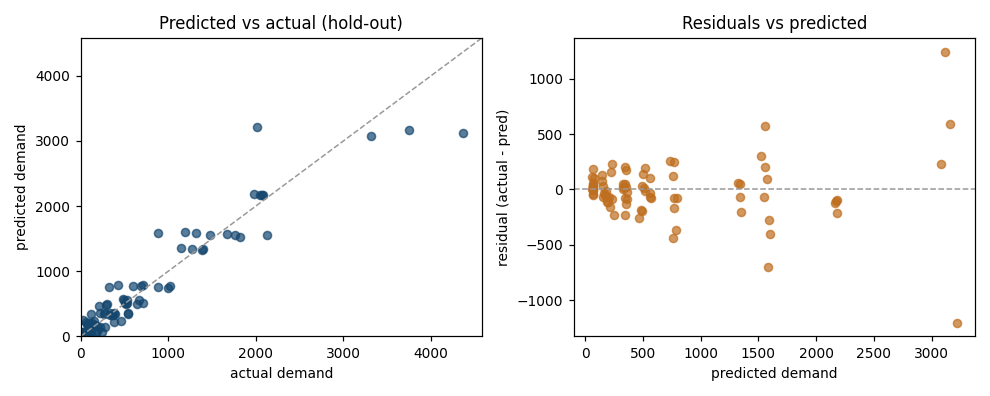
\includegraphics[width=0.92\textwidth]{../../figuras/m1_residuos_modelo.png}
\end{center}

% ============================================================
\section{Limites e próximos passos}
\begin{itemize}
    \item \textbf{Janela curta:} 19 meses (15 de treino) é pouco para caracterizar sazonalidade anual; a conclusão ``sem sinal temporal explorável'' vale para esta janela e deve ser revista com mais histórico.
    \item \textbf{Teste de 4 meses:} diferenças de $\sim$0,4~pp em WAPE estão dentro do ruído amostral; por isso ``empate'' é leitura correta, não ``vitória marginal''.
    \item \textbf{A base registra desfechos, não sinais antecedentes:} o que prediz bem a demanda (tratamentos ativos/iniciados no próprio mês) é contemporâneo ao alvo, logo vazamento; defasá-lo remove o vazamento e também o sinal.
    \item \textbf{Perspectivas investigadas:} regressão com features internas (empata), classificação de suspensão (não acionável) e features derivadas~+~dados públicos externos (clima/epidemiologia) --- documentadas em \texttt{docs/}.
\end{itemize}

\section*{Uso de IA generativa}
\sloppy
Assistente de IA usado para apoio à investigação de \emph{features}, estruturação do \emph{pipeline} (\texttt{Pipeline}\slash\texttt{ColumnTransformer}, \emph{baselines}, avaliação) e redação. As decisões de formulação, unidade, partição, métrica e escolha de modelo são da equipe. Nenhum dado pessoal de paciente foi inserido em serviço externo. Nenhum número foi inventado --- todos vêm de execução real sobre \texttt{data/raw/}.

% ============================================================
{\footnotesize
\begin{thebibliography}{9}
\setlength{\itemsep}{0pt}
\bibitem{springer2026} \emph{Hospital trust network features inform ML for medicines demand forecasting.} Springer, Discover Applied Sciences, 2026.
\bibitem{lightgbm2021} \emph{Optimising hospital pharmacy inventory for high-value, intermittent-demand drugs (LightGBM-Tweedie).} 2021.
\bibitem{hyndman2006} Hyndman \& Koehler. \emph{Another look at measures of forecast accuracy (MASE).} Int.\ J.\ Forecasting, 2006.
\bibitem{m4comp} Makridakis et al. \emph{The M4/M5 Competitions: results, findings, conclusions.} Int.\ J.\ Forecasting, 2018/2022.
\bibitem{sample2019} \emph{Sample size and relative ML forecasting performance.} arXiv:1909.13316.
\bibitem{conformal2026} \emph{A training-free conformal interval is a strong forecasting baseline.} arXiv:2606.09473, 2026.
\bibitem{forecastability} \emph{How to Assess Forecastability (sample entropy / AMI).} 2009; arXiv:2601.10006.
\bibitem{captopril2025} De Meo \& Gonçalves. \emph{Comparing time series techniques for medication demand forecasting (captopril, São Paulo).} DGO 2025.
\end{thebibliography}
}

\end{document}
